\section{Natural Language Processing (NLP)}
\subsection{The 4 Key-Ingredients of Machine Learning}
\textbf{1. Data (Input)}
\begin{itemize}
    \item Dataset (Input-Vektor), bestehend aus Features ($X$) und Labels ($Y$).
    \item Pre-Processing Pipe-Line including cleansing, feature-engineering, data augmentation etc.
    \begin{itemize}
        \item \textbf{cleansing}: identifying and correcting errors in the dataset. z.B. Rechtschreibefehler in Text erkennen und korrigieren (mögliches korrektes Wort vorschlagen)
        \item \textbf{feature-engineering}: the process of using domain knowledge to extract features (characteristics, properties, attributes) from raw data. Nicht nur Rohdaten, sondern auch noch Features extrahieren (nicht nur Katze vorschlagen, sondern auch Verbindung von Katze zu Säugetier herstellen). Damit ML Modell mit Features weiterarbeiten kann (z.B. Wörter in One-Hot-Rep. darstellen)
        \item \textbf{Data-Augumentation}: Man hat gewisse Daten (z.B. Sammlung von Katzenfotos), damit man gut Machine-learning machen kann benötigt man viele Daten $\rightarrow$ vorhandene Bilder manipulieren (schwarz/weiss, spiegeln, etc.) um aus einem Bild möglichst viele andere zu erstellen damit man mehr Inputs hat
    \end{itemize}
\end{itemize}
\textbf{2. Cost-Function (Loss)}
\begin{itemize}
    \item Formal mathematical expression for good / bad
    \item Commonly Mean Squared Error (MSE)
    \item \textit{Beispiel}: 2 Fotos vorhanden (Katzen und Hunde) $\rightarrow$ wenn Katze als Hund erkannt wird, ist das sehr schlecht und muss dem Computer mitgeteilt werden (Mathematische Funktion wie gut oder schlecht Ergebnis war)
    \item auch Fehler oder Residual genannt (Differenz zwischen Vorhersage $\hat{y}$ und Wirklichkeit $y$ )
\end{itemize}
\textbf{3. Model}
\begin{itemize}
    \item From linear model: $\hat{y_i} = ax_i + b$
    \item To complicated million parameter neural networks
    \item Different tasks require different models (regression / decision tree)
    \item Aus einem Input wird (über eine mathematische Funktion) ein Output generiert
\end{itemize}
\textbf{4. Optimization Procedure (Optimizer)}
\begin{itemize}
    \item Algorithm that changes the parameters of the model that the cost-function is minimized.
    \item E.g. \textit{Stochastic Gradient Descent (SGD), ADAM, RMSProp...}
    \item Model Trainieren mit verschiedenen Parametern, etc.
\end{itemize}

\subsection{More ingredients}
For successful ML, there are many more ingredients:\\ 
\textbf{5. Performance optimization}
\begin{itemize}
    \item Building of efficient pipe-lines
    \item Folowing tool specific recommendations
\end{itemize}
\textbf{6. Visualization and evaluation of the learning Process}
\begin{itemize}
    \item Learning curves
    \item Performance measures
    \item Tensorboard
\end{itemize}
\textbf{7. Cross-Validation \& Regularization}
\begin{itemize}
    \item Train models that generalize well to unseen data
    \item Estimate the generalization error
\end{itemize}

\subsection{Representation of Words}
Vectors can be used to represent words based on their meaning.
\subsubsection{One-hot representation/ One-hot Encoding}
\begin{itemize}
    \item Vector with a single 1-Value
    \item All other Values are set to 0
    \item Skalarprodukt von Vektoren ergibt IMMER 0
    \item Count the Number of different Words, Define one unique vector per word:
\end{itemize}
\textit{Dini Mom isch fett.}\\
Dini: $\begin{bmatrix} \textcolor{red}{1}\\ 0\\ 0\\ 0\\ 0\end{bmatrix}$
Mom: $\begin{bmatrix} 0\\ \textcolor{red}{1}\\ 0\\ 0\\ 0\end{bmatrix}$
isch: $\begin{bmatrix} 0\\ 0\\ \textcolor{red}{1}\\ 0\\ 0\end{bmatrix}$
fett: $\begin{bmatrix} 0\\ 0\\ 0\\ \textcolor{red}{1}\\ 0\end{bmatrix}$
'.': $\begin{bmatrix} 0\\ 0\\ 0\\ 0\\ \textcolor{red}{1}\end{bmatrix}$\\ 
\textbf{Disadvantages:}
\begin{itemize}
    \item Very high dimensional vector space (1 Dimension / unique Word)
    \item Sparse Representation: Eech vector has a single 1 and $N$ Zeroes. (Memory Inefficient)
    \item No Generalization: All words are unrelated to each other.
    \item Does not capture any aspect of the meaning of a word
\end{itemize}

\subsubsection{Indexing}
Make a list of words (optionally alphabetically). Use the index to represent each word.\\ 
\textbf{Example:}\\
\textit{Dini Mom isch fett.}\\ 
Dini: $0$, Mom: $1$, isch: $2$, fett: $3$, '.': $4$
\begin{itemize}
    \item Dense Equivalent of one-hot encoding
    \item Indexes are not more useful that one-hot vectors
    \item Often used as preprocessing step
    \item Indices / One-Hot Vectors are fed into a network which learns more useful representations
\end{itemize}

\subsubsection{Distributed Representation}
\begin{itemize}
    \item Words that occur in similar contexts (neighboring words) tend to have similar meanings
    \item Similar words share similar representations
    \item Distributed representations can be learned
\end{itemize}
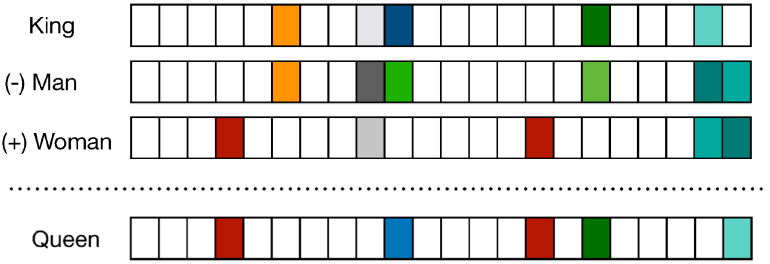
\includegraphics[width=.8\linewidth]{./img/distributed_representation.png}\\
\textbf{Words to Vectors:}
\begin{itemize}
    \item Mathematical function maps word to high dimensional Vector
    \item In neural networks, this function is implemented in the Embedding Layer
\end{itemize}
\textbf{Advantage of Vectors}
\begin{itemize}
    \item Good embedding maps simiar/related words to similar regions of the vector space
    \item Dot-Product (Skalarprodukt) is a measure of similarity
    \item Possible to add/subtract vectors
\end{itemize}
\textbf{Calculate Similarities between words}
Dot-Product (Skalarprodukt) of 2 Vectors:
\begin{itemize}
    \item maximal when parallel (0\textdegree) (1 with norm (length) 1)
    \item zero when orthogonal/ senkrecht (90\textdegree)
    \item minimal (negative) when opposite directions (180\textdegree) (-1 with norm (length) 1)
\end{itemize}
\textbf{Why make it sense to normalize the vector representations \TODO{allenfalls normalisieren erklären}}
\begin{itemize}
    \item Skalarprodukt wird auf 1 "Normalisiert" $\rightarrow$ somit muss Skalarprodukt in Formel nicht mehr ausgerechnet werden
    \item damit norm-Vektor nicht immer neu ausgerechnet werden muss, sondern nur noch verwendet werden kann
\end{itemize}
\textbf{Cosine Distance}
\begin{itemize}
    \item Way to calculate how similar two words (vectors) are
\end{itemize}
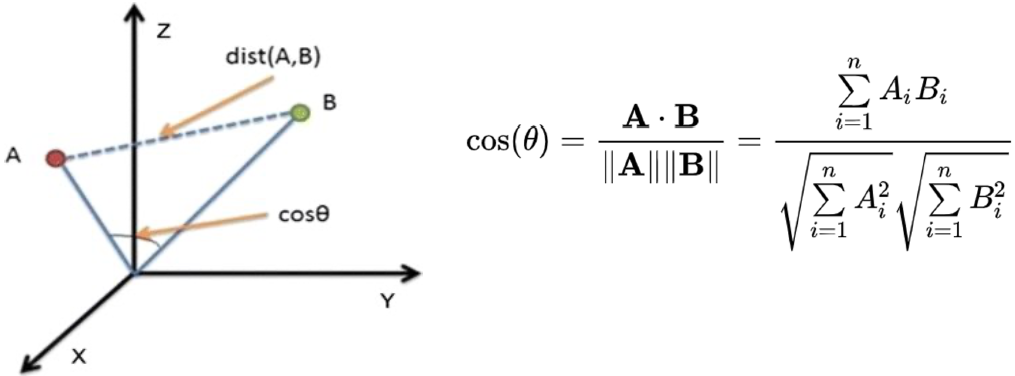
\includegraphics[width=\linewidth]{./img/cosine_distance.png}

\subsubsection{Cosine-Distance vs. Cosine-Similarity}
\begin{itemize}
    \item cosine similarity is a similarity metric between vectors
    \item Je grösser die Cosine-Distanz wird, desto kleiner wird auch die Cosine-Similarity
    \item Je kleiner die Cosine-Distanz wird, desto höher wird auch die Cosine-Similarity
    \item Je kleiner $cos(\theta)$, desto höher die Similarity \& desto kleiner  die Distance
    \begin{itemize}
        \item \textit{Cosine similarity range}: $-1$ meaning exactly opposite, 1 meaning exactly the same, 0 indicating orthogonality (senkrecht)
    \end{itemize} 
    \item if 2 vectors are perfectly the same then similarity is 1 (angle=0) and thus, distance is 0 (1-1=0)
    \item \textbf{Cosine-Similarity}: $cos(\theta) = \frac{a * b}{|a|*|b|} \rightarrow$ Winkel zwischen $P_1$ \& $P_2$
    \item \textbf{Cosine-Distance}: $1 - CosineSimilarity$
\end{itemize}